% Figure of doc/frame_format.md (build.sh turns page 1 into frame.svg)
\documentclass[tikz,border=8pt]{standalone}
\usepackage{xcolor}
\pagecolor{white}
\usetikzlibrary{positioning,decorations.pathreplacing,calc,arrows.meta}
% colors and styles shared by the figures of doc/
\definecolor{hdr}{HTML}{FFF2B3}   % size and other headers
\definecolor{tok}{HTML}{C9DCF5}   % tokens, joint symbols
\definecolor{lit}{gray}{0.86}      % literals
\definecolor{off}{HTML}{FAD7B5}   % offset fields
\definecolor{ext}{HTML}{CDEBC7}   % extensions and extra bits
\definecolor{flg}{HTML}{F2A65A}   % flags
\definecolor{endm}{HTML}{F5C2C2}  % end markers
\definecolor{tab}{HTML}{E3D5F2}   % code tables
\definecolor{b1}{HTML}{FBE3CC}    % one, two, three offset bytes
\definecolor{b2}{HTML}{F5BE8A}
\definecolor{b3}{HTML}{E8914A}
\tikzset{
  fld/.style={draw, minimum height=9mm, inner sep=2pt, align=center},
  brc/.style={decorate, decoration={brace, amplitude=4pt}},
  mbrc/.style={decorate, decoration={brace, mirror, amplitude=4pt}}}

\begin{document}

%% 1. frame: a WZ frame
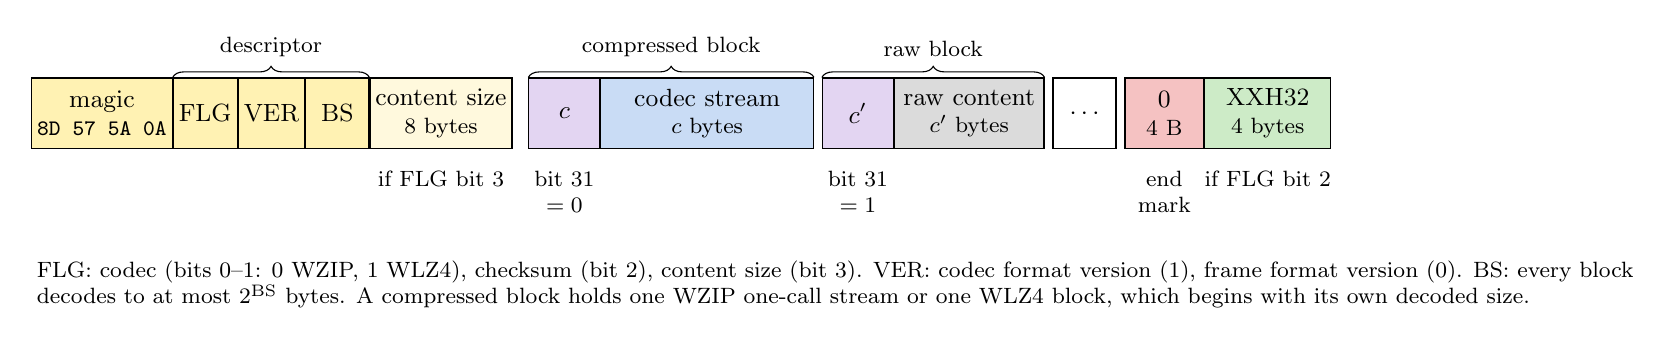
\begin{tikzpicture}[font=\small, node distance=0pt]
\node[fld, fill=hdr, minimum width=17mm, align=center] (m) at (0.85,0) {magic\\[-1pt]\footnotesize\texttt{8D 57 5A 0A}};
\node[fld, fill=hdr, minimum width=8mm, right=of m] (f) {FLG};
\node[fld, fill=hdr, minimum width=8mm, right=of f] (v) {VER};
\node[fld, fill=hdr, minimum width=8mm, right=of v] (b) {BS};
\node[fld, fill=hdr!45, minimum width=17mm, right=of b, align=center] (cs) {content size\\[-1pt]\footnotesize 8 bytes};
\node[fld, fill=tab, minimum width=9mm, right=2mm of cs, align=center] (h1) {$c$};
\node[fld, fill=tok, minimum width=27mm, right=of h1, align=center] (d1) {codec stream\\[-1pt]\footnotesize $c$ bytes};
\node[fld, fill=tab, minimum width=9mm, right=1mm of d1, align=center] (h2) {$c'$};
\node[fld, fill=lit, minimum width=19mm, right=of h2, align=center] (d2) {raw content\\[-1pt]\footnotesize $c'$ bytes};
\node[fld, minimum width=8mm, right=1mm of d2] (dots) {$\cdots$};
\node[fld, fill=endm, minimum width=10mm, right=1mm of dots, align=center] (e) {0\\[-1pt]\footnotesize 4 B};
\node[fld, fill=ext, minimum width=16mm, right=of e, align=center] (x) {XXH32\\[-1pt]\footnotesize 4 bytes};
\draw[brc] (f.north west) -- (b.north east) node[midway, above=4pt, font=\footnotesize] {descriptor};
\draw[brc] (h1.north west) -- (d1.north east) node[midway, above=4pt, font=\footnotesize] {compressed block};
\draw[brc] (h2.north west) -- (d2.north east) node[midway, above=4pt, font=\footnotesize] {raw block};
\node[below=1.5mm of cs, font=\footnotesize, align=center] {if FLG bit 3};
\node[below=1.5mm of x, font=\footnotesize, align=center] {if FLG bit 2};
\node[below=1.5mm of e, font=\footnotesize, align=center] {end\\mark};
\node[below=1.5mm of h1, font=\footnotesize, align=center] {bit 31\\$=0$};
\node[below=1.5mm of h2, font=\footnotesize, align=center] {bit 31\\$=1$};
\node[anchor=north west, font=\footnotesize, align=left] at (-0.1,-1.75) {FLG: codec (bits 0--1: 0 WZIP, 1 WLZ4), checksum (bit 2), content size (bit 3).
VER: codec format version (1), frame format version (0). BS: every block\\decodes to at most $2^{\mathrm{BS}}$ bytes. A compressed block holds one WZIP one-call stream or one WLZ4 block, which begins with its own decoded size.};
\end{tikzpicture}

\end{document}
